\chapter{Comment les animaux se reproduisent}\label{ch:g4:animal-reproduction}

En mai, la mare résonne du chant des grenouilles~; en juin, elle est
noire de \omterm{ex:g2:animals-grow-up:frog}{têtards}. Le chant, on le découvre, était le début de
l'histoire~: la reproduction --- la façon dont les \omterm{def:g1:animals-around-us:animal}{animaux}
fabriquent la génération suivante --- suit des règles qui valent de
la grenouille à l'éléphant, avec de merveilleuses variantes dans le
détail.

\section{Il en faut deux}

\begin{definition}[Reproduction sexuée]\label{def:g4:animal-reproduction:sexual}
Chez les \omterm{def:g1:animals-around-us:animal}{animaux}, faire des petits demande le plus souvent deux
parents~: une \emph{femelle}\index{femelle} et un
\emph{mâle}\index{mâle}. La femelle produit des \emph{cellules
œufs}\index{cellule œuf}~; le mâle produit des \emph{cellules
mâles}\index{cellule mâle}. Un jeune \omterm{def:g1:animals-around-us:animal}{animal} commence lorsqu'une
cellule mâle rejoint une cellule \omterm{def:g2:animals-grow-up:born}{œuf} --- cette rencontre est la
\emph{fécondation}\index{fécondation}. La reproduction à deux
parents s'appelle la \emph{reproduction
sexuée}\index{reproduction sexuée}.
\end{definition}

\begin{example}[Pourquoi les grenouilles chantent]\label{ex:g4:animal-reproduction:song}
Le chœur de mai, ce sont les \omterm{def:g4:animal-reproduction:sexual}{mâles} qui appellent les \omterm{def:g4:animal-reproduction:sexual}{femelles} à la
mare. Chaque couple libère ensuite ses cellules dans l'eau --- les
\omterm{def:g2:animals-grow-up:born}{œufs} de la \omterm{def:g4:animal-reproduction:sexual}{femelle}, les \omterm{def:g4:animal-reproduction:sexual}{cellules mâles} du \omterm{def:g4:animal-reproduction:sexual}{mâle} --- et c'est là que
se produit la \omterm{def:g4:animal-reproduction:sexual}{fécondation}. Les points noirs dans la gelée, quelques
jours plus tard, sont les jeunes qui grandissent déjà~: le chant
était la première étape du cycle de la grenouille de
\cref{ch:g2:animals-grow-up}.
\end{example}

\begin{omfigure}
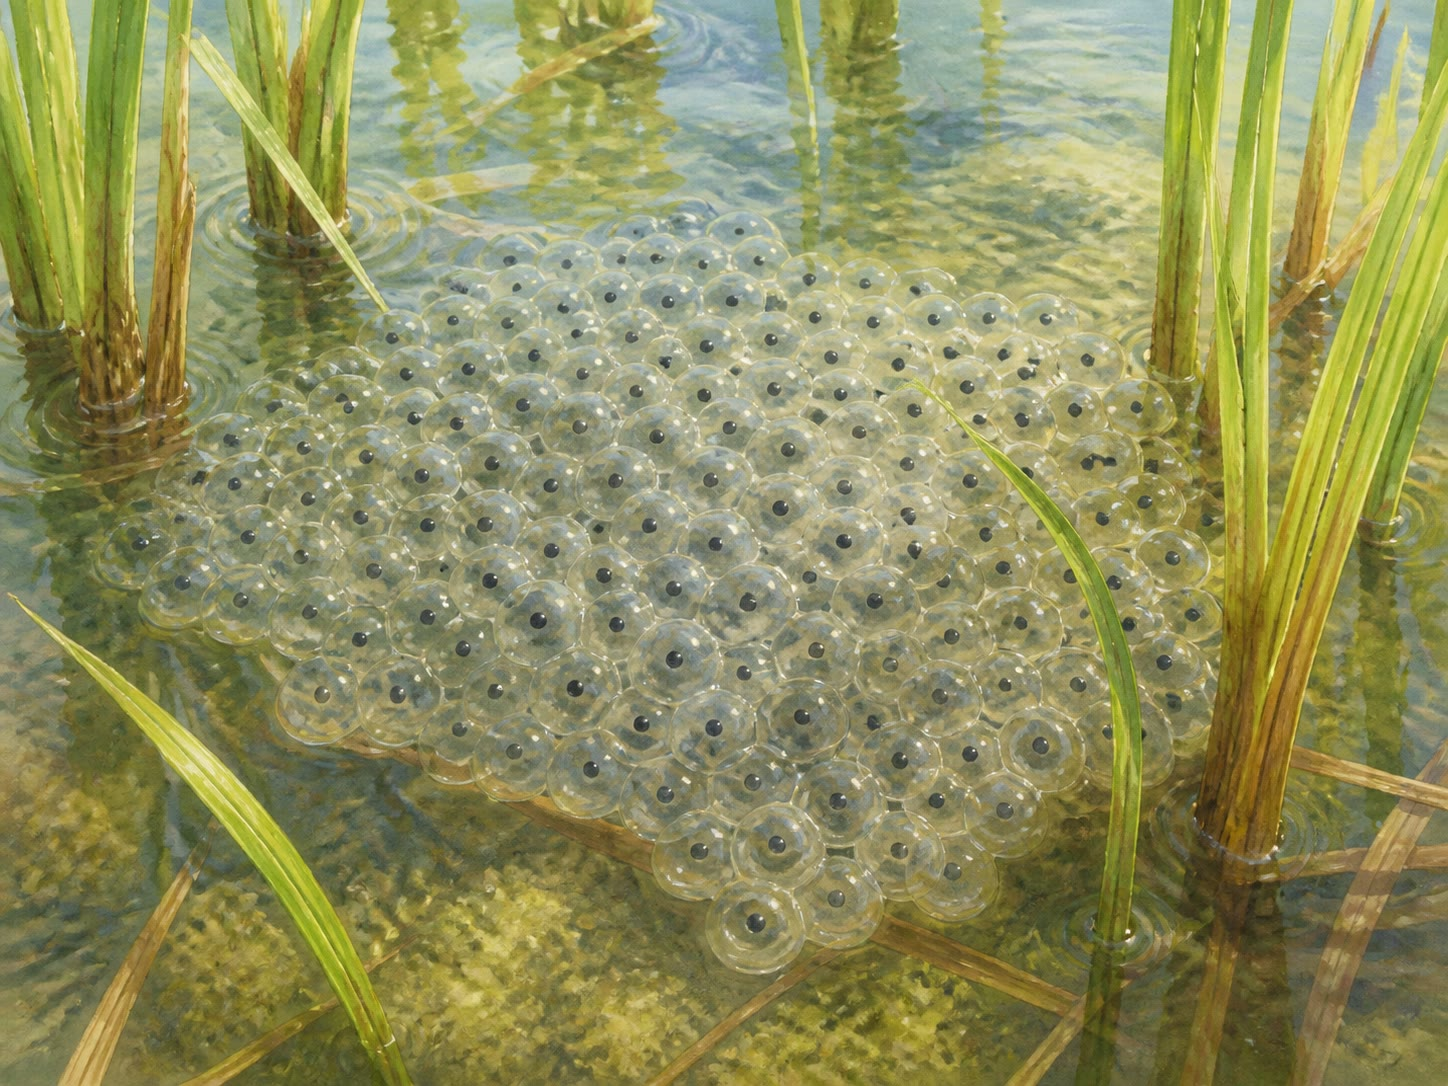
\includegraphics[width=0.56\linewidth]{images/book1/ai/g4-repro-frogspawn.jpg}

{\small Quelques jours après le chœur~: de la ponte de grenouille
parmi les roseaux, chaque sphère de gelée étant un \omterm{def:g2:animals-grow-up:born}{œuf} fécondé où
commence une jeune grenouille.}
\end{omfigure}

\begin{remark}[Deux parents, une chance mêlée]\label{rem:g4:animal-reproduction:mix}
Un jeune \omterm{def:g1:animals-around-us:animal}{animal} reçoit quelque chose de chacun de ses parents ---
c'est pourquoi un poulain peut avoir la robe de sa mère et la liste
blanche de son père. Ce que chaque parent transmet exactement, et
comment, est l'une des grandes questions qui attendent dans ce
livre~; pour l'instant, retiens simplement que tout \omterm{def:g1:animals-around-us:animal}{animal} issu de
la \omterm{def:g4:animal-reproduction:sexual}{reproduction sexuée} a deux parents et ressemble aux deux.
\end{remark}

\section{Œufs pondus, ou petits nés vivants}

\begin{definition}[Ovipare et vivipare]\label{def:g4:animal-reproduction:ovivivi}
Les deux façons de naître de \cref{def:g2:animals-grow-up:born}
reçoivent maintenant leurs noms scientifiques~:
\begin{itemize}
  \item un \omterm{def:g1:animals-around-us:animal}{animal} est \emph{ovipare}\index{ovipare} si la \omterm{def:g4:animal-reproduction:sexual}{femelle}
        pond des \emph{\omterm{def:g2:animals-grow-up:born}{œufs}} et si les jeunes achèvent leur
        croissance dans l'\omterm{def:g2:animals-grow-up:born}{œuf}, hors de son corps~: \omterm{prop:g3:sorting-living-things:groups}{oiseaux}, la
        plupart des \omterm{prop:g3:sorting-living-things:groups}{poissons}, la plupart des \omterm{prop:g4:classifying-animals:classes}{reptiles}, \omterm{prop:g3:sorting-living-things:groups}{amphibiens},
        \omterm{prop:g3:sorting-living-things:groups}{insectes}, escargots~;
  \item un \omterm{def:g1:animals-around-us:animal}{animal} est \emph{vivipare}\index{vivipare} si le jeune
        grandit \emph{dans le corps de la mère}, nourri par elle,
        et \emph{naît vivant}~: presque tous les \omterm{prop:g3:sorting-living-things:groups}{mammifères}.
\end{itemize}
\end{definition}

\begin{example}[Deux nurseries]\label{ex:g4:animal-reproduction:nurseries}
Le poussin de la poule passe trois semaines au chaud dans un \omterm{def:g2:animals-grow-up:born}{œuf} à
\omterm{def:g1:animals-around-us:covering}{coquille}, en vivant du jaune
(\cref{rem:g2:animals-grow-up:egg})~; le poulain passe onze mois
dans la jument, nourri sans arrêt par son corps, et naît prêt à
tenir debout dans l'heure. Même but, deux nurseries~: un
casse-croûte emporté dans une \omterm{def:g1:animals-around-us:covering}{coquille}, un service en chambre à
l'intérieur.
\end{example}

\begin{proposition}[Où se produit la fécondation]\label{prop:g4:animal-reproduction:where}
Chez les habitants de l'eau comme les \omterm{prop:g3:sorting-living-things:groups}{poissons} et les grenouilles,
la \omterm{def:g4:animal-reproduction:sexual}{fécondation} se produit couramment \emph{dans l'eau}, hors du
corps de la \omterm{def:g4:animal-reproduction:sexual}{femelle} --- \omterm{def:g2:animals-grow-up:born}{œufs} et \omterm{def:g4:animal-reproduction:sexual}{cellules mâles} sont libérés ensemble
et se rencontrent par milliers. Chez les \omterm{def:g1:animals-around-us:animal}{animaux} terrestres ---
\omterm{prop:g3:sorting-living-things:groups}{oiseaux}, \omterm{prop:g4:classifying-animals:classes}{reptiles}, \omterm{prop:g3:sorting-living-things:groups}{mammifères}, \omterm{prop:g3:sorting-living-things:groups}{insectes} --- les cellules
sécheraient à l'air libre~; le \omterm{def:g4:animal-reproduction:sexual}{mâle} dépose donc ses cellules
\emph{dans le corps de la \omterm{def:g4:animal-reproduction:sexual}{femelle}} au cours de
l'\emph{accouplement}\index{accouplement}, et la \omterm{def:g4:animal-reproduction:sexual}{fécondation} s'y
produit.
\end{proposition}
\admitted

\section{Peu de petits très soignés, ou beaucoup et pas du tout}

\begin{proposition}[Deux stratégies pour la génération suivante]\label{prop:g4:animal-reproduction:strategies}
Compare les nombres~: une morue libère des \emph{millions} d'\omterm{def:g2:animals-grow-up:born}{œufs}
par an et n'en soigne aucun~; une éléphante a \emph{un} petit tous
les quelques années et le garde une dizaine d'années. Entre ces deux
extrêmes, une règle vaut dans tout le monde \omterm{def:g1:animals-around-us:animal}{animal}~: plus une espèce
produit de jeunes, moins chacun reçoit de soins --- et moins elle en
produit, plus chacun est protégé et nourri. Les deux stratégies
réussissent~: en moyenne, assez de jeunes survivent pour remplacer
les parents.
\end{proposition}
\admitted

\begin{example}[Compter la mare]\label{ex:g4:animal-reproduction:pondcount}
La ponte d'un seul couple de grenouilles contient des milliers
d'\omterm{def:g2:animals-grow-up:born}{œufs}. Hérons, épinoches et larves de libellule (voir
\cref{ex:g3:food-chains:three}) mangent des \omterm{ex:g2:animals-grow-up:frog}{têtards} tout le
printemps --- et sur ces milliers, une poignée de grenouillets
grimpe sur la berge en juillet. L'énorme ponte n'est pas du
gaspillage~: c'est la réponse de la grenouille aux dangers de la
mare, sans la moindre garde parentale.
\end{example}

\begin{example}[L'autre extrême]\label{ex:g4:animal-reproduction:whalecalf}
Le baleineau naît seul, nage aussitôt à côté de sa mère, boit son
\omterm{def:g2:animals-grow-up:born}{lait} très riche pendant de longs mois et est défendu contre tous les
dangers. Un seul petit à la fois --- mais celui-là reçoit tout. Les
\omterm{prop:g3:sorting-living-things:groups}{mammifères}, avec leur \omterm{def:g2:animals-grow-up:born}{lait}
(\cref{def:g2:animals-grow-up:born}), sont les grands spécialistes
de la stratégie du «~peu et bien soignés~».
\end{example}

\begin{method}[Lire la stratégie d'une espèce]\label{met:g4:animal-reproduction:read}
Devant une espèce, demande-toi~:
\begin{enumerate}
  \item Combien de jeunes à la fois --- un, une douzaine, des
        milliers~?
  \item Qui les garde et les nourrit --- les deux parents, la mère,
        personne~?
  \item Où commencent-ils --- dans un \omterm{def:g2:animals-grow-up:born}{œuf} à l'extérieur, ou
        grandis à l'intérieur~?
  \item Vérifie l'équilibre de
        \cref{prop:g4:animal-reproduction:strategies}~: beaucoup de
        jeunes peu soignés, ou peu de jeunes très soignés.
\end{enumerate}
\end{method}

\section{Exercices}

\begin{exercise}[$\star$]\label{exo:g4:animal-reproduction:1}
Qu'est-ce que la \omterm{def:g4:animal-reproduction:sexual}{fécondation}~? Quelle cellule vient de chaque
parent~?
\end{exercise}

\begin{exercise}[$\star$]\label{exo:g4:animal-reproduction:2}
Définis \omterm{def:g4:animal-reproduction:ovivivi}{ovipare} et \omterm{def:g4:animal-reproduction:ovivivi}{vivipare}, avec deux \omterm{def:g1:animals-around-us:animal}{animaux} de chaque sorte.
\end{exercise}

\begin{exercise}[$\star$]\label{exo:g4:animal-reproduction:3}
Pourquoi les grenouilles chantaient-elles en mai~? Raconte
l'histoire de la mare en trois étapes.
\end{exercise}

\begin{exercise}[$\star$]\label{exo:g4:animal-reproduction:4}
Où se produit la \omterm{def:g4:animal-reproduction:sexual}{fécondation} chez la truite, et où chez la poule~?
Pourquoi cette différence, d'après
\cref{prop:g4:animal-reproduction:where}~?
\end{exercise}

\begin{exercise}[$\star$]\label{exo:g4:animal-reproduction:5}
Compare les nurseries du poussin et du poulain~: où grandit chacun,
et qu'est-ce qui le nourrit~?
\end{exercise}

\begin{exercise}[$\star$]\label{exo:g4:animal-reproduction:6}
Énonce la règle qui relie le nombre de jeunes aux soins qu'ils
reçoivent. Donne les deux exemples extrêmes du chapitre.
\end{exercise}

\begin{exercise}[$\star$]\label{exo:g4:animal-reproduction:7}
Les millions d'\omterm{def:g2:animals-grow-up:born}{œufs} de la morue ne deviennent presque jamais des
morues adultes. Pourquoi la stratégie réussit-elle quand même~?
\end{exercise}

\begin{exercise}[$\star$]\label{exo:g4:animal-reproduction:8}
Applique \cref{met:g4:animal-reproduction:read} à la chatte~: une
portée typique d'environ cinq petits, allaités et gardés par la mère
pendant des semaines, grandis en elle. De quel côté de la balance
est-elle~?
\end{exercise}

\begin{exercise}[$\star\star$]\label{exo:g4:animal-reproduction:9}
Un poulain ressemble souvent à ses deux parents à la fois. Que
montre cela sur ce que reçoit le jeune, d'après
\cref{rem:g4:animal-reproduction:mix}~?
\end{exercise}

\begin{exercise}[$\star\star$]\label{exo:g4:animal-reproduction:10}
Le \omterm{def:g4:animal-reproduction:sexual}{mâle} de l'épinoche construit un nid, ventile les \omterm{def:g2:animals-grow-up:born}{œufs} et chasse
les intrus --- un dévouement rare chez un poisson. À l'aide de
\cref{prop:g4:animal-reproduction:strategies}, que prédirais-tu sur
la taille de sa ponte, comparée aux millions de la morue~?
\end{exercise}

\begin{exercise}[$\star\star\star$]\label{exo:g4:animal-reproduction:11}
Les tortues marines rampent sur la plage pour enterrer leurs \omterm{def:g2:animals-grow-up:born}{œufs}
dans le sable chaud, puis retournent à la mer. \omterm{def:g4:animal-reproduction:ovivivi}{Ovipares} ou
\omterm{def:g4:animal-reproduction:ovivivi}{vivipares}~? Soignées ou non~? Et pourquoi ce reptile, nageur toute
sa vie, doit-il quand même pondre sur la \emph{terre ferme}~?
(Sers-toi des caractères des \omterm{prop:g4:classifying-animals:classes}{reptiles} de
\cref{prop:g4:classifying-animals:classes}.)
\end{exercise}
